\documentclass[12pt]{report}
\usepackage{graphicx}
\usepackage{parskip}
\usepackage{needspace}
\usepackage[hidelinks]{hyperref}

\begin{document}
\tableofcontents

%%%%%%%%%%%%%%%%%%%%%%%%%%%%%%%%%%%%%%%%%%%%%%%%%%%%%%%%%%%%%%%%%%%%%%%%%%%%%%%
\chapter{User Guide} \label{UserGuide}

\begin{figure}[htb]
    \centering
    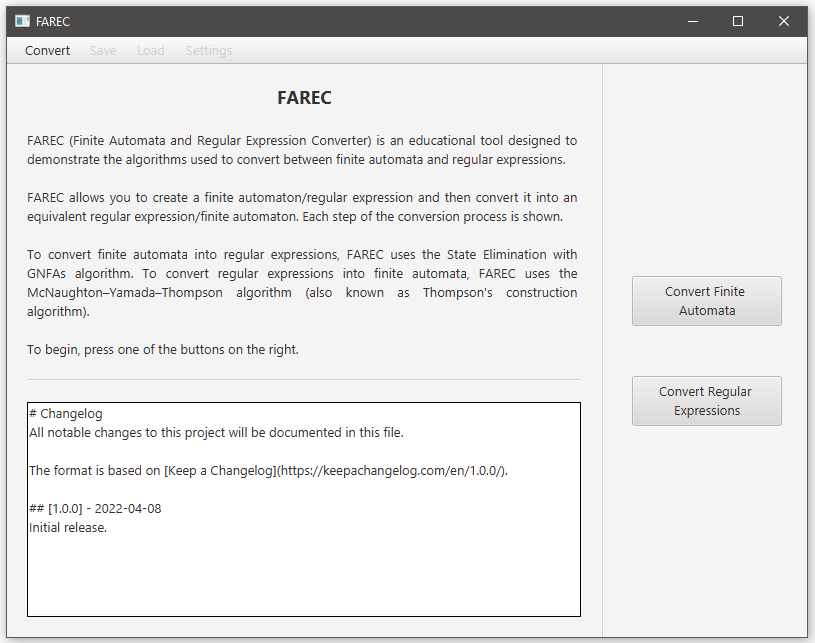
\includegraphics[width=\textwidth]{./Diagrams/StartScreen.png}
    \caption{The start screen is displayed upon starting the program.}
    \label{StartScreen}
\end{figure}

\needspace{2em}

Once you have launched FAREC, you will be greeted by the start screen, shown in
Figure~\ref{StartScreen}. The start screen contains a welcome message, a
changelog showing the latest entry and two buttons. The Convert Finite Automata
button will take you to the finite automata creation screen, where you can
create finite automata to convert into regular expressions. The Convert Regular
Expressions button will take you to the regular expression creation screen,
where you can create regular expressions to convert into finite automata.

Throughout the application, a menu bar is available at the top of the window.
This menu contains two menu items which have the same functionality as the two
buttons found in the start screen.

%%%%%%%%%%%%%%%%%%%%%%%%%%%%%%%%%%%%%%%%%%%%%%%%%%%%%%%%%%%%%%%%%%%%%%%%%%%%%%%
\section{Creating Finite Automata} \label{CreatingFiniteAutomata}

\begin{figure}[htb]
    \centering
    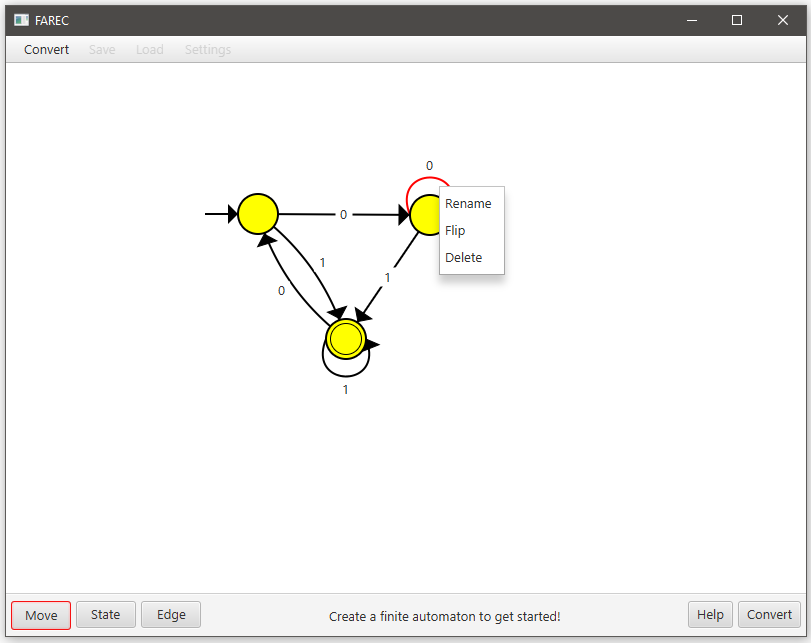
\includegraphics[width=\textwidth]{./Diagrams/CreateFAScreen.png}
    \caption{The finite automata creation screen allows you to create finite
    automata to convert into regular expressions.}
    \label{CreateFAScreen}
\end{figure}

The finite automata creation screen allows you to create finite automata to
convert into regular expressions. The workspace in the centre is where you
create the finite automata. At the bottom of the screen there is a toolbar with
several buttons and a small text area. The text area will display tips and error
messages. The three buttons on the left are used to change between work modes.
You can also change between work modes by using the number keys on the keyboard.
There are three available work modes:

\begin{enumerate}
    \item In the \textbf{Move} work mode, you can move states around the
    workspace by holding left-click and dragging. Moving states past the bottom
    and right boundaries of the workspace will increase its size. Once the
    workspace has expanded, you can use the scroll bars or hold left-click and
    pan on the workspace to move the view.
    \item In the \textbf{State} work mode, left-clicking on the workspace will
    create a new state.
    \item In the \textbf{Edge} work mode, you can create edges between states.
    To create an edge between two states, hold left-click while on top of the
    start state and then release while on top of the end state. To create a loop
    edge, the start and end state should be the same state. There can only be
    one edge in each direction between any two states.
\end{enumerate}

Regardless of the work mode, right-clicking a state or edge will open its
context menu. This allows you to perform various actions. States can be renamed,
deleted, set as initial states and set as final states. Note that there can be
only one initial state and only one final state, and they cannot be the same
state. Edges can be renamed and deleted. Loop edges can also be flipped to
change their position. 

States can be given any name. Any states that you do not name will be
automatically named by the program once the automaton is complete. Edges can
only be named using Latin alphanumeric characters. You can have several
characters on an edge label, by writing them as a comma separated list.

The Help button on the right side of the toolbar will open a help window that
contains useful information to help you create finite automata. Once your finite
automaton is complete, press the Convert button. This will open the finite
automata conversion screen. Make sure that your finite automaton is valid: it
must have an initial state, a final state, and all states must be reachable from
the initial state.

%%%%%%%%%%%%%%%%%%%%%%%%%%%%%%%%%%%%%%%%%%%%%%%%%%%%%%%%%%%%%%%%%%%%%%%%%%%%%%%
\section{Converting Finite Automata} \label{ConvertingFiniteAutomata}

\begin{figure}[htb]
    \centering
    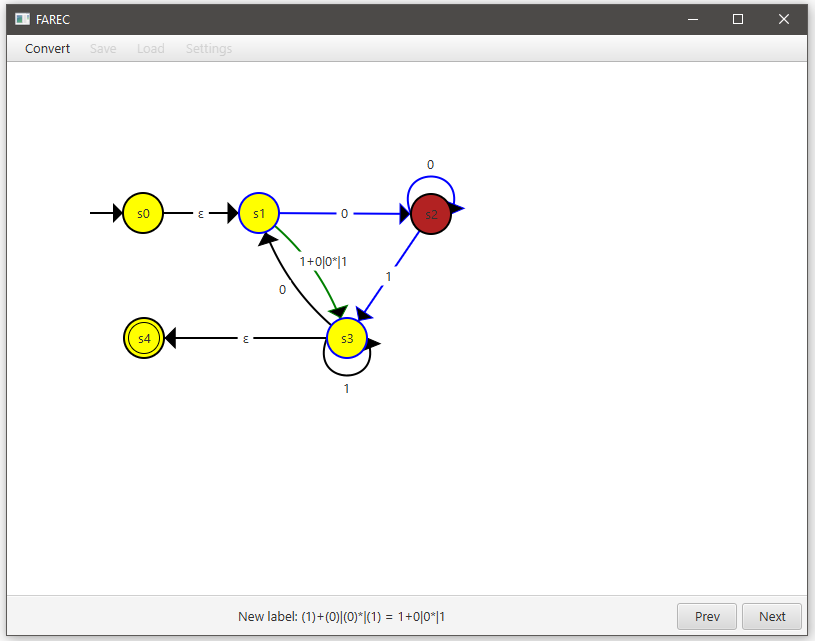
\includegraphics[width=\textwidth]{./Diagrams/ConvertFAScreen.png}
    \caption{The finite automata conversion screen allows you to convert finite
    automata into regular expressions.}
    \label{ConvertFAScreen}
\end{figure}

The finite automata conversion screen allows you to convert finite automata into
regular expressions. Once again there is a workspace where the finite automaton
is displayed. The toolbar at the bottom has another text area, as well as two
buttons for moving backwards and forwards through the conversion process. The
text area will display instructions as well as information about the conversion
process.

The conversion process consists of three stages that may be repeated several
times.

\begin{enumerate}
    \item In the \textbf{Select} stage, you select a state to remove from the
    finite automaton. This is done by left-clicking on the state and then
    pressing the Next button. The state selected will be marked with a red
    color. The initial and final states cannot be removed.
    \item In the \textbf{Update} stage, the labels on the edges of the finite
    automaton are updated to reflect the imminent removal of the selected state.
    The edge currently being updated is highlighted green. States and edges that
    are involved in the update are highlighted blue. The process of creating the
    new label is shown in the text area in the toolbar. The simplified new label
    is shown on the edge.
    \item In the \textbf{Remove} stage, the selected state is removed from the
    finite automaton. If there are no more states to remove, the process will
    end and the regular expression equivalent to the finite automaton will be
    displayed in the text area in the toolbar. Otherwise, the process goes back
    to the Select stage and the cycle repeats.
\end{enumerate}

%%%%%%%%%%%%%%%%%%%%%%%%%%%%%%%%%%%%%%%%%%%%%%%%%%%%%%%%%%%%%%%%%%%%%%%%%%%%%%%
\section{Creating Regular Expressions} \label{CreatingRegularExpressions}

\begin{figure}[htb]
    \centering
    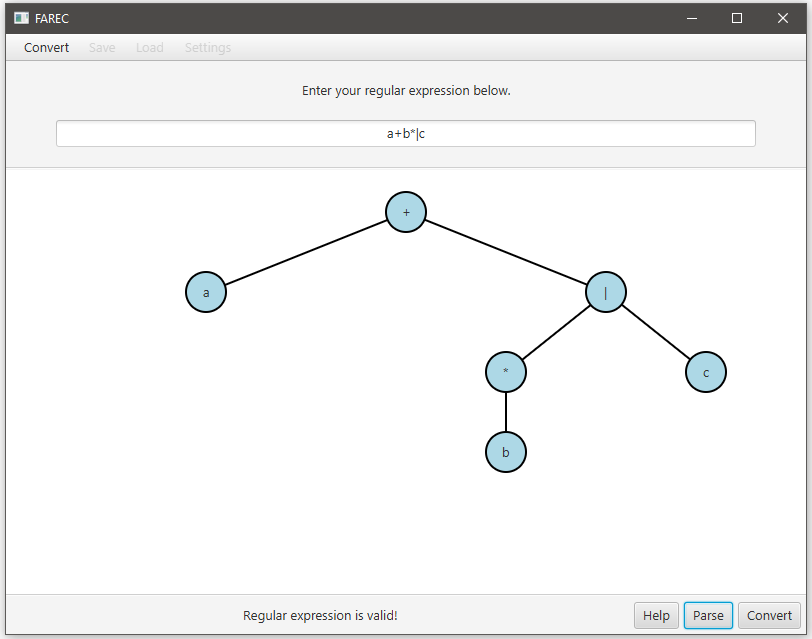
\includegraphics[width=\textwidth]{./Diagrams/CreateREScreen.png}
    \caption{The regular expression creation screen allows you to create regular
    expressions to convert into finite automata.}
    \label{CreateREScreen}
\end{figure}

The regular expression creation screen allows you to create regular expressions
to convert into finite automata. Regular expressions are created by typing them
into the text field at the top of the screen. Regular expressions can only
contain Latin alphanumeric characters, regex operators, brackets and whitespace.
There are three regex operators available:

\begin{itemize}
    \item The \textbf{Kleene} star operator can be used by typing the asterisk
    \textbf{*} symbol.
    \item The \textbf{concatenation} operator can be used by typing the vertical
    pipe \textbf{$|$} symbol. If your keyboard does not have this symbol, you
    can enter it by holding down Alt and typing 124 on the numeric keypad of
    your keyboard.
    \item The \textbf{union} operator can be used by typing the plus \textbf{+}
    symbol.
\end{itemize}

The Help button on the right side of the toolbar will open a help window that
contains useful information to help you create regular expressions. Once your
regular expression is complete, press the Parse button. If the expression is
valid, its parse tree will be displayed. You can then convert the regular
expression into a finite automaton by pressing the Convert button. This will
open the regular expression conversion screen. If your regular expression is
invalid, the text area in the toolbar will tell you what and where the problem
is.

%%%%%%%%%%%%%%%%%%%%%%%%%%%%%%%%%%%%%%%%%%%%%%%%%%%%%%%%%%%%%%%%%%%%%%%%%%%%%%%
\section{Converting Regular Expressions} \label{ConvertingRegularExpressions}

\begin{figure}[htbp]
    \centering
    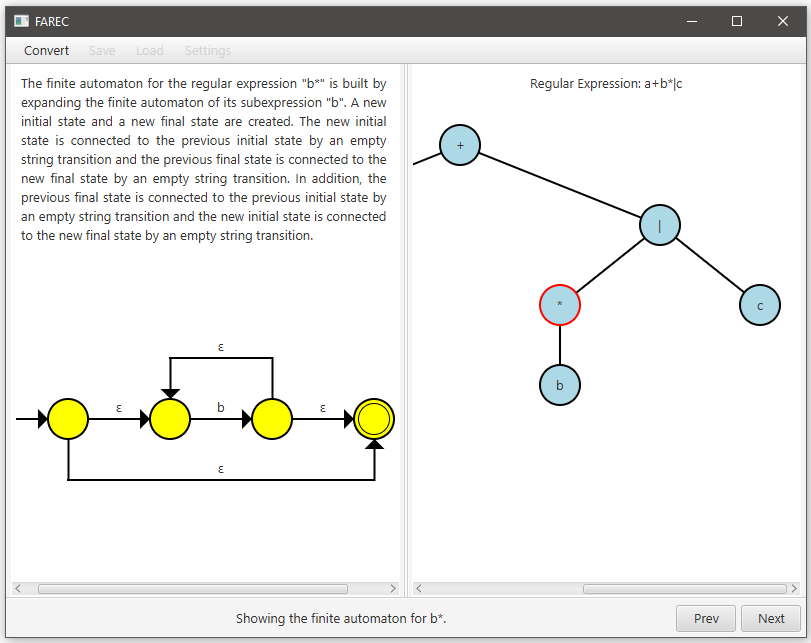
\includegraphics[width=\textwidth]{./Diagrams/ConvertREScreen.png}
    \caption{The regular expression conversion screen allows you to convert
    regular expressions into finite automata.}
    \label{ConvertREScreen}
\end{figure}

The regular expression conversion screen allows you to convert regular
expressions into finite automata. The screen is split into two halves. The left
half displays the finite automaton built for the current regular expression, as
well as a short text explaining how the finite automaton was constructed. The
right half shows the regular expression you created in the previous screen, as
well as its parse tree. The node of the parse tree that is currently being
considered is highlighted red. The text area in the toolbar at the bottom of the
screen shows the regular expression for this node (and by extension for the
finite automaton being built). The toolbar also contains two buttons for moving
backwards and forwards through the conversion process.

\end{document}
